%%%%%%%%%%%%%%%%%%%%%%%%%%%%%%%%%%%%%%%%%%%%%%%%%%%%%%%%%%%%%%%%%%%%%%%%%%%

\documentclass{standalone}

\usepackage{amsmath}
\usepackage{mathptmx}
\usepackage{pgfplots}
\usetikzlibrary{external}
\tikzexternalize{frond12-estimated-b}
\pgfplotsset{compat=1.15}

%% IEEE uses Times Roman font, so we'll default to Times.
%% These three commands make up the entire times.sty package.
\renewcommand{\rmdefault}{ptm}
\renewcommand{\ttdefault}{pcr}
\normalfont\selectfont

\begin{document}

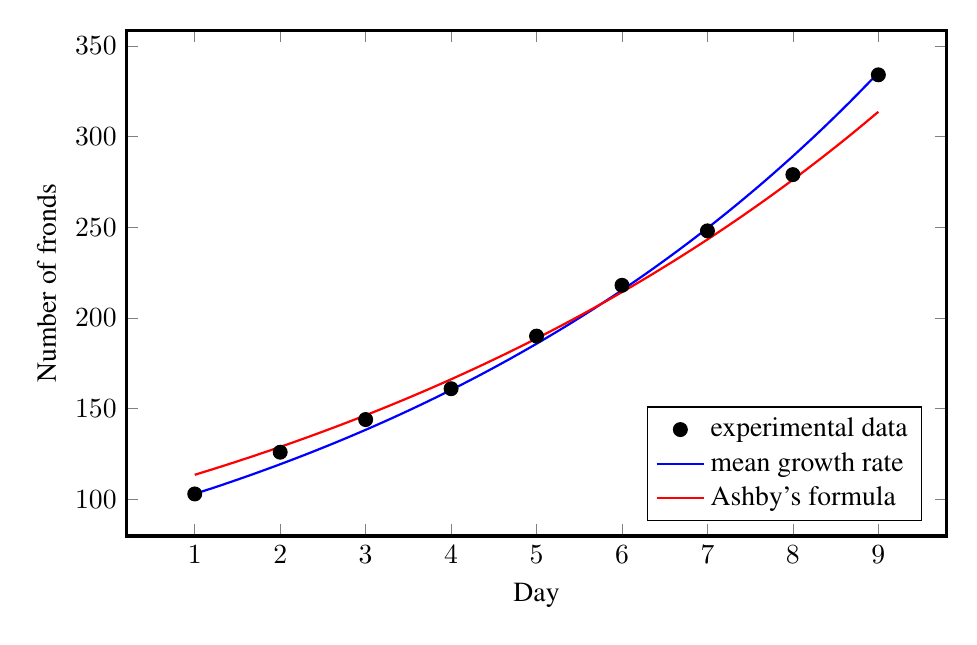
\begin{tikzpicture}
\tikzset{%%
  every mark/.append style={scale=1.0},%%
  scale=1.0%%
}
\pgfplotsset{%%
  every axis/.append style={font=\normalsize}%%
}
%%
\begin{axis}[%%
  axis line style=very thick,%%
  dotStyle/.style={mark size=2.5,black,mark color=black,mark=*,only marks},%%
  enlargelimits=true,%%
  height=8cm,%%
  legend cell align=left,%%
  legend pos=south east,%%
  plotStyle/.style={%%
    domain=1:9,%%
    mark=none,%%
    smooth,%%
    thick%%
  },%%
  width=12cm,%%
  %% x axis
  xlabel={\normalsize Day},%%
  %% y axis
  ylabel={\normalsize Number of fronds},%%
  scaled y ticks=false,%%
  y tick label style=/pgf/number format/fixed%%
]
%%
%%
\addplot[dotStyle] coordinates {
  (1, 103)
  (2, 126)
  (3, 144)
  (4, 161)
  (5, 190)
  (6, 218)
  (7, 248)
  (8, 279)
  (9, 334)
};
\addlegendentry{experimental data}
%%
%%
\addplot+ [plotStyle,blue]
{103*(1.158932^(x-1))};
\addlegendentry{mean growth rate}
%%
%%
\addplot+ [plotStyle,red]
{100*exp(0.127*x)};
\addlegendentry{Ashby's formula}
\end{axis}
\end{tikzpicture}

\end{document}
